\documentclass[12pt, reqno]{amsart}

\usepackage[
a4paper,% other options: a3paper, a5paper, etc
margin = 2.5cm
% use vmargin=2cm to make vertical margins equal to 2cm.
% us  hmargin=3cm to make horizontal margins equal to 3cm.
% use margin=3cm to make all margins  equal to 3cm.
]
{geometry}

\usepackage{amsmath}
\usepackage{amsfonts}
\usepackage{amsthm}
\usepackage{amssymb}
\usepackage{graphicx}
\usepackage{ulem}

\title{Modelling Disease Spread - Midterm Checkpoint}
\author{(Group 10) Subhodh Kotekal, Dongil Lee, Hongyang Li, Boyuan Yu}
\date{November 13, 2020}
\linespread{1.25}

\begin{document}
    \maketitle

    \section{Introduction to the SIR model}

    The Susceptible-Infected-Removed Model for Disease Spread, in which we will call it the SIR model in the following discussion, is a model that puts each individual in the population into exactly one of three catagories: \(S\), \(I\) and \(R\). In the simplest setting of simulating a disease spread, the \(S\) category contains those individuals who are susceptible to the disease. Meanwhile, the \(I\) category stands for the infected individuals who can spread the disease, and the \(R\) category is the population of "removed" individuals who were previously infected, and are no longer able to spread the disease. In reality, one can think of the \(R\) category as people who have either recovered and immuned to the disease, or died. We also want to introduce two parameters \(b\) and \(k\). The parameter \(b\) represents the number of people that an infected individual spreads disease to through interaction each day, and \(k\) is the fraction of infected population that is "removed" (become members in the \(R\) category). Together, we can formulate this model in to a system of odinary differential equations, where \(s(t)\), \(i(t)\) and \(r(t)\) denote the size of the population of the corresponding category as a funtion of time variable \(t\) as the following:
    \begin{align*}
        s'(t) &= -b\cdot s(t) \cdot i(t) \\
        i'(t) &= b \cdot s(t) \cdot i(t) - k\cdot i(t) \\
        r'(t) &= k \cdot i(t).
    \end{align*}
One can interpret the equations as follows: the first equation shows that the number of susceptible people who are newly infected (hence being moved from \(S\) category to \(I\) category) at each given time is positively correlated with \(s(t)\), \(i(t)\) and parameter \(b\). Intuitively speaking, it means more people would be infected each day if there are more susceptible people, more infected people, or more interactios between populations. The third equation shows that the number of infected people being removed (hence being moved from \(I\) category to \(R\) category) at each given time is positively correlated with \(i(t)\) and parameter \(k\). It means that more people would be removed (or recovered) each day if there are more infected people or higher rate of "removing" (or recovery). The second equation can be seen as a result of the first and the third equation, as the sum of population of categories must be equal to the total population N at any given time.

    \section{Structure of \texttt{sir}}

    To conduct simulations of ODE version of the SIR model, we take an object oriented approach by creating the \texttt{SIR\_ODE} class. A \texttt{SIR\_ODE} object can be created by providing the parameters \texttt{b} and \texttt{k} as well as providing the initial data \texttt{i(0)} and the population size \texttt{N}. This object thus stores the parameters of a model of interest, and the object can be made to simulate the solution for a given interval of time. The parameters of the \texttt{SIR\_ODE} can be easily changed. The purpose of this object is to neatly package all of the information of a particular instantiation of the SIR model. This \texttt{SIR\_ODE} object is the primitive representation of the ODE version of the SIR model. Variants of the SIR model that will be used in the final project will be associated to corresponding objects that inherit from \texttt{SIR\_ODE}. 

    To Build a discrete version of the SIR model, we also take an object oriented approach by first creating the \texttt{SIR\_DISCRETE} class, which represents a person with three states: 'S', 'I', and 'R'. The person's state can be obtained and assigned. Then we initialize the simulation by providing the population size \texttt{N} and initial infected and susceptible people ratio: \texttt{$i_0$} and \texttt{$s_0$}. The simulation precedes by updating the states based on two parameters: \texttt{k} and \texttt{b}. Further variations for final project can be implemented by either inheriting from the existing class or changing the way to update states of people.
    \section{Preliminary investigations}

    To get a first sense of how the ODE version of the SIR model behaves, we started with a simple simulation. We considered the parameter configuration of \(k = 0.05, b = 10, N = 10000\) and \(i_0 = 0.0001\). In words, about \(5\%\) of those infected recover per day, there are about \(10\) interactions per day per individual that could spread the disease, the population size is \(10000\) individuals, and \(0.01\%\) of the population is infected at time \(0\). Using the \texttt{solve\_ivp} function from \texttt{scipy}, we simulate the solution of \(S(t), I(t), R(t)\) for \(0 \leq t \leq 50\) and obtain Figure \ref{fig:simulation0}. With this configuration of parameters, the dynamics are striking in how fast the number of infected individuals rises. In particular, the number of susceptible people in the population drops to zero extremely quickly. The mirroring dynamics of the infected and recovered individuals agrees with intuition. 

    \begin{figure}
        \centering
        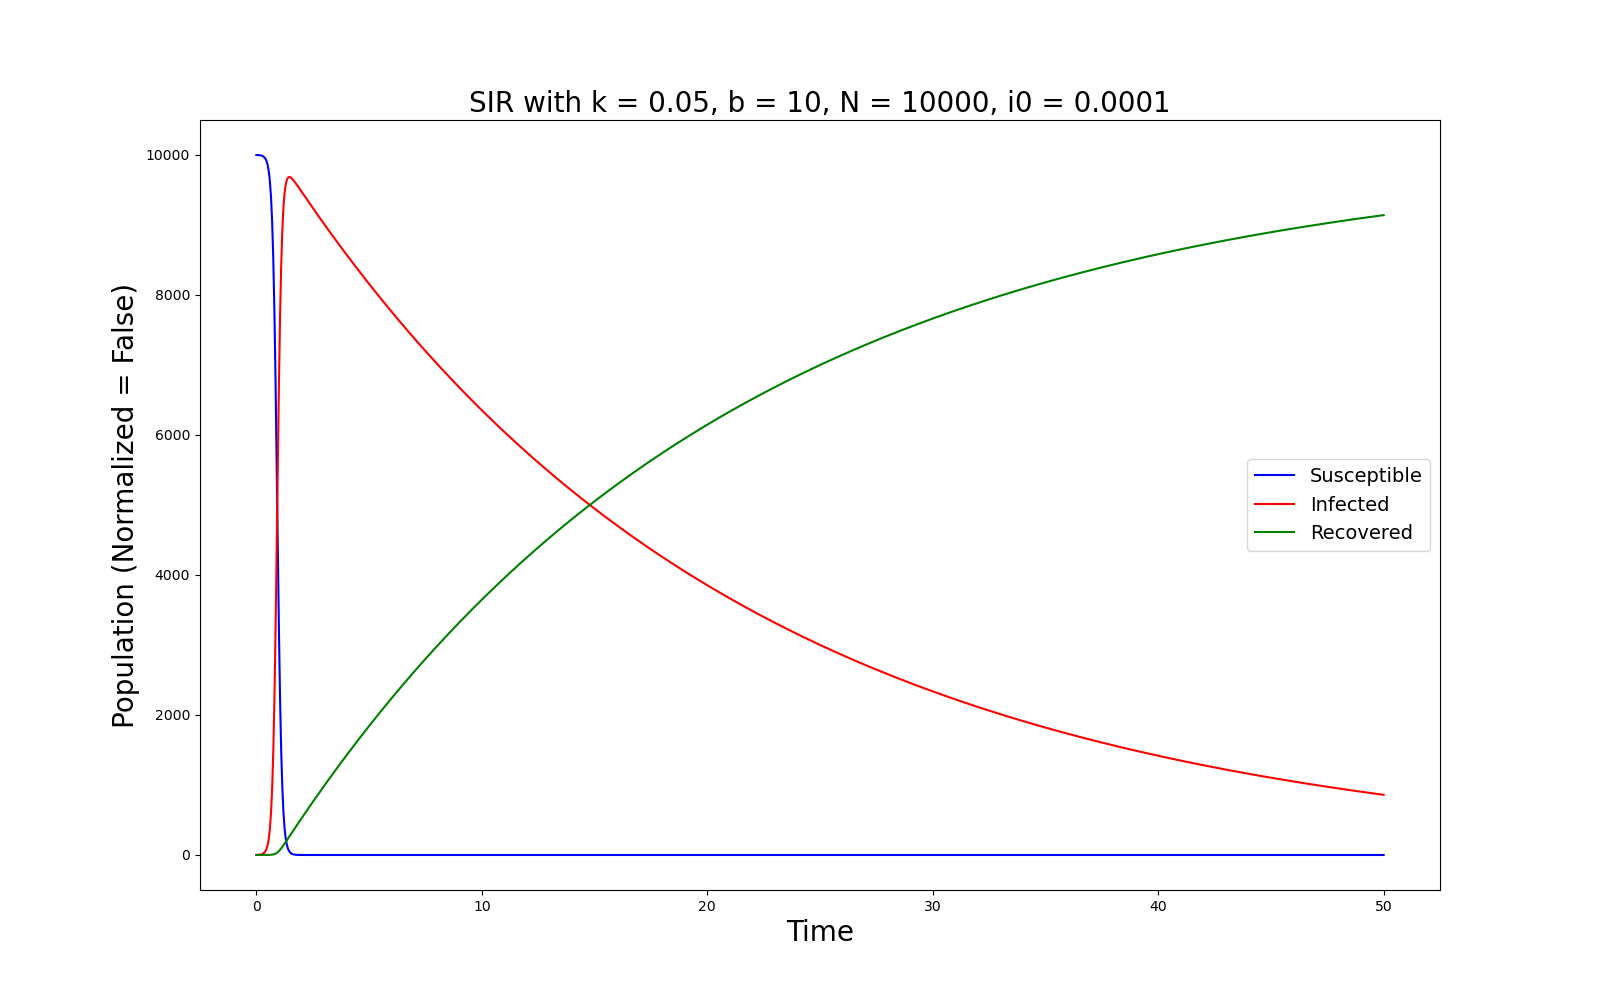
\includegraphics[scale=0.8]{sir_ode_simulation0.png}
        \caption{A simulation of a SIR model.}
        \label{fig:simulation0}
    \end{figure}

    We suspect that the reason for the such rapid increase increase is due to the choice of \(b = 10\). To examine how social distancing might affect the dynamics, we ran the same simulation, except now we set \(b = 1\). There is only one interaction per day per individual in this socially distanced society. The dynamics corresponding to this ODE system is given in Figure \ref{fig:simulation1}. These dynamics are quite different from those seen in Figure \ref{fig:simulation0}. We immediately notice that the time it takes for \(S(t)\) to drop to zero is about ten times as long in Figure \ref{fig:simulation1} than it is in Figure \ref{fig:simulation0}. Furthermore, we see that the highest number of infected people is much lower in Figure \ref{fig:simulation1} than it is in Figure \ref{fig:simulation0}. As expected from the equations of the SIR model, the growth rate of \(R(t)\) is the same in both figures. The parameter \(b\) dictates not only the rate at which susceptible individuals become infected, but also the peak of the total number of infected people at any given time. This relationship between \(b\) and the height of the red curve (\(I(t)\)) is perhaps what is behind the idea of ``flattening the curve'' via social distancing. 
    
    \begin{figure}
        \centering
        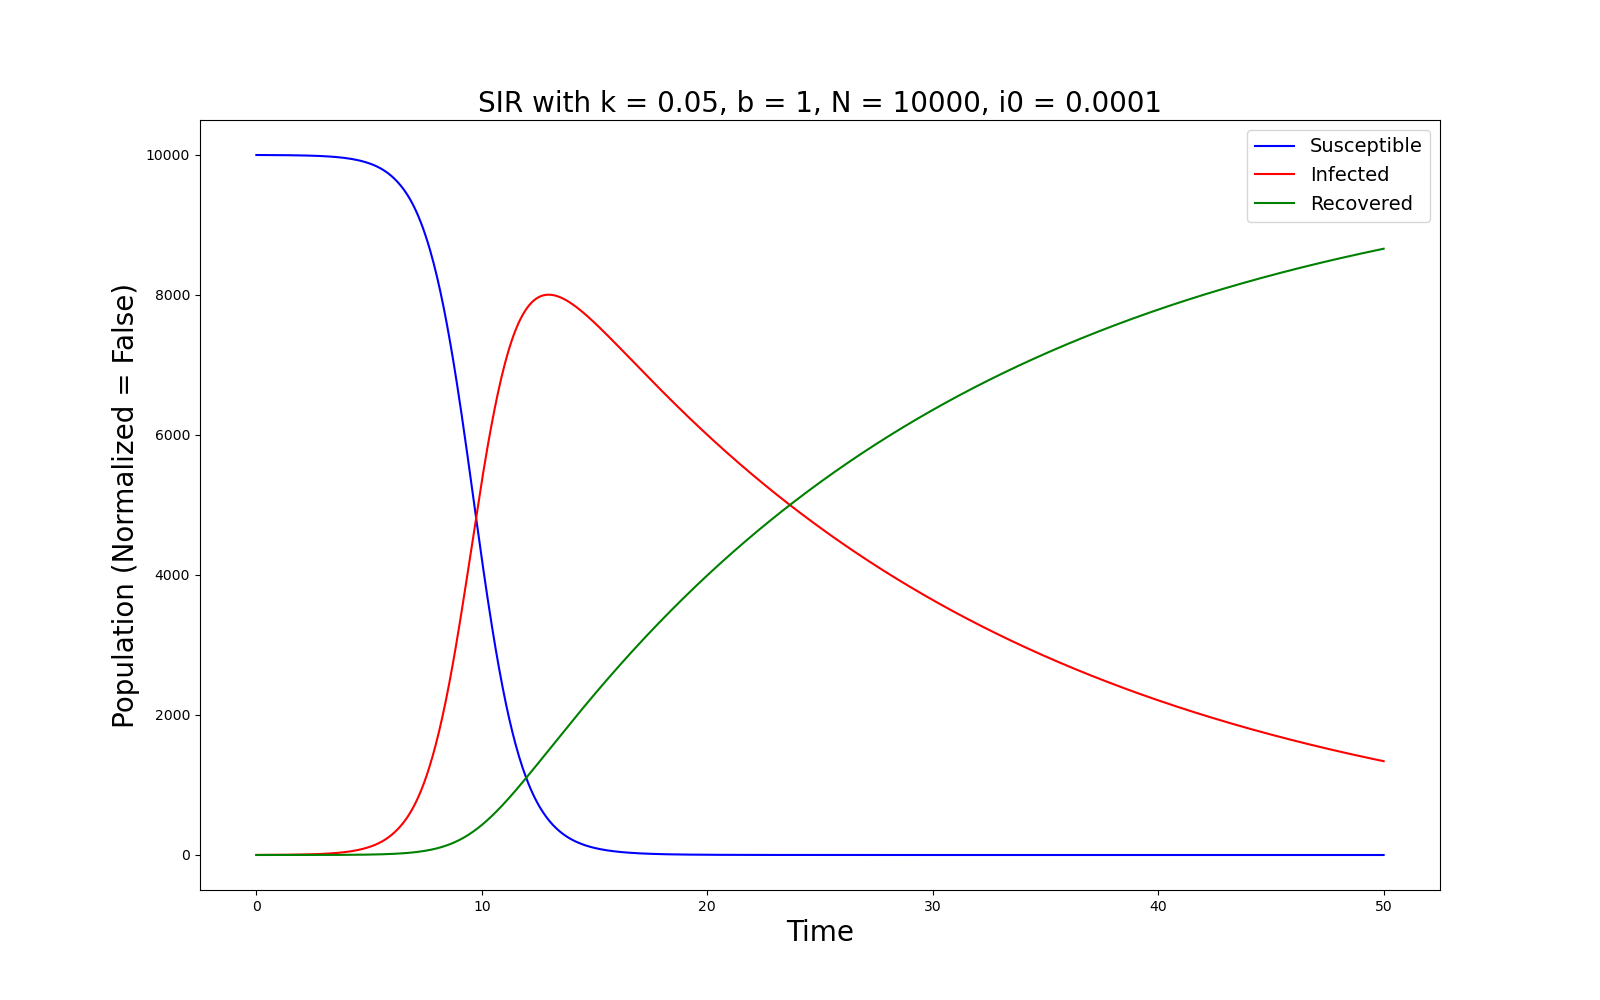
\includegraphics[scale=0.8]{sir_ode_simulation1.png}
        \caption{A simulation of an SIR model in a ``socially distanced'' society.}
        \label{fig:simulation1}
    \end{figure}

    We investigate further how the interplay between \(b\) and \(k\) can affect qualitative features of the dynamics. We first examine how the parameters affect the time it takes for all individuals to have been infected at some point (i.e. how do the parameters affect \(t^*\) where \(t^*\) is the earliest time that \(S(t) = 0\)). Running many simulations over different configurations of \(b\) and \(k\), we obtain the phase transition diagram in Figure \ref{fig:phase_transition_full_infection}. The phase transition diagram agrees with basic intuition. Generally speaking, the time to full infection decreases as \(b\) increases. Further, the time to full infection decreases as \(k\) decreases. For low values of \(b\) and larger values of \(k\), there is actually never a time that \(S(t) = 0\). In other words, there are people in the population who never have been infected. Note that low values of \(b\) and larger values of \(k\) correspond to situations where people engage in social distancing for a disease that most people can recover quickly from. As such, such a parameter configuration is not very realistic. However, it is interesting to see that strict social distancing measures do work when recovery rates are small (i.e. low values of both \(b\) and \(k\)). In the lower left hand corner of the phase diagram, we do see that small \(b\) can lead to scenarios in which some people never get infected.

    \begin{figure}
        \centering
        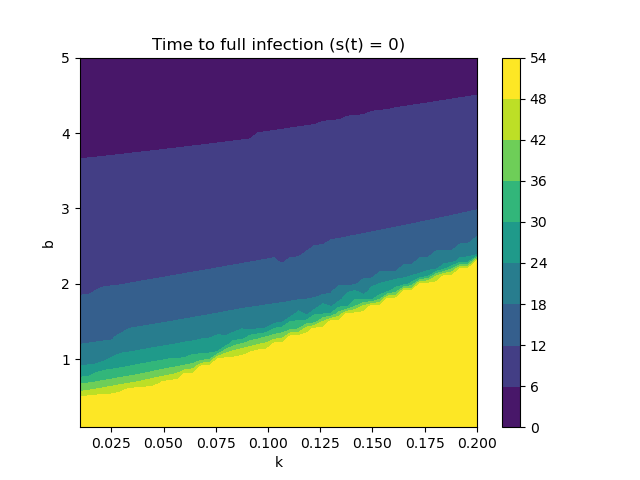
\includegraphics[scale=0.8]{phase_transition_full_infection.png}
        \caption{Phase diagram relating parameters and time to full infection.}
        \label{fig:phase_transition_full_infection}
    \end{figure}

    We also investigate how the choice of \(b\) and \(k\) affects the time to which over half the population is infected and not recovered (\(i(t) > 0.5\)). Such situations are severe ones in which the hospital system is overburdened with the tremendous number of active infections. While this event is related to the event in which \(S(t) = 0\), investigating the time at which \(i(t) > 0.5\) gives a more transparent indication to the severity of the outbreak. After all, there are many situations in which everyone may become infected but we always have \(i(t) < 0.5\). This investigation thus sheds light on which parameter configurations yield severe outcomes. Running the simulation over many configurations of the parameters, we obtain the phase diagram in Figure \ref{fig:phase_transition_outnumber}.

    While the phase diagram in Figure \ref{fig:phase_transition_outnumber} is similar to the diagram in Figure \ref{fig:phase_transition_full_infection}, it must be noted that the yellow region is shifted down (note the scale for \(b\) is different in the two plots). The diagram agrees with basic intuition. When \(b\) is small and \(k\) is large, there is low spread of disease from infected members to susceptible members, and many infected members are quickly recovering. The story is the same as in 3 for the other phase diagram regions as well. As we mentioned before, it's interesting to see that the yellow region is shifted down compared to Figure \ref{fig:phase_transition_full_infection}. This result is surprising in that we had originally thought that there may be situations in which \(s(t)\) hits zero yet \(i(t) < 0.5\) always. Instead, it seems that the reverse is much more likely, in that \(i(t) > 0.5\) is achieved yet \(s(t) > 0\) always. This is seen in the regions that are yellow in Figure \ref{fig:phase_transition_full_infection} and non-yellow in 4 (often \(b\) is moderate). 

    \begin{figure}
        \centering
        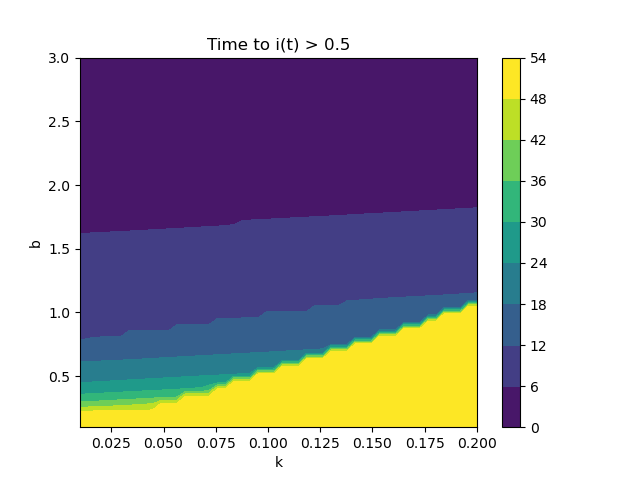
\includegraphics[scale=0.8]{phase_transition_outnumber.png}
        \caption{Phase diagram relating parameters and time to \(i(t) > 0.5\).}
        \label{fig:phase_transition_outnumber}
    \end{figure}
    
    \newpage
    
     We now switch to discrete SIR model and run simulations to see if discrete and continuous models agree on the dynamics of disease spread. We start by using the same set of parameters that resulted in Figure \ref{fig:simulation0} for our first discrete simulation. From Figure \ref{fig:discrete_simulation0}, we can see that the discrete model is in agreement with the ODE version in terms of its overall projection on how the state of the individuals will change over time. In particular, the number of infected reaches its peak at around the same time and susceptible people quickly drops to zero as shown in ODE model. The "mirroring dynamics" of the infected and the recovered observed in Figure \ref{fig:simulation0} remains largely the same as well. A small difference is that the curves for discrete model are not as smooth as the ODE version since both the Time and number of people in different states change in discrete fashion. 
    
    \begin{figure}[h]
        \centering
        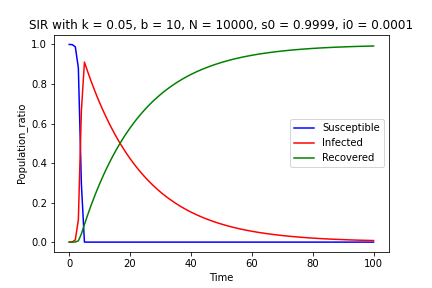
\includegraphics[scale=0.8]{sir_discrete_simulation0.png}
        \caption{A simulation of discrete SIR model.}
        \label{fig:discrete_simulation0}
    \end{figure}
    
    Next, we investigate whether the discrete model agrees or disagrees with the continuous model on how the number of interactions each person makes per day on average influences the dynamics of disease spread. In particular, we are interested in seeing if the discrete model will produce a different projection on the efficacy of social distancing on slowing down the spread of infectious disease. Running the same simulation with the parameter b now set to 1 instead of 10, as in ODE social distancing simulation, we obtain Figure \ref{fig:discrete_simulation1}. Except for quantitative details such as exactly when the maximum number of infected people are reached and how quickly people get infected or recovered, Figure  \ref{fig:simulation1} and Figure \ref{fig:discrete_simulation1} are qualitatively very similar; it tells us that social distancing is an effective measure in fighting the infectious disease by 'flattening the curve' (as represented by the slope with which the red curve reaches its peak).
    \begin{figure}[h]
        \centering
        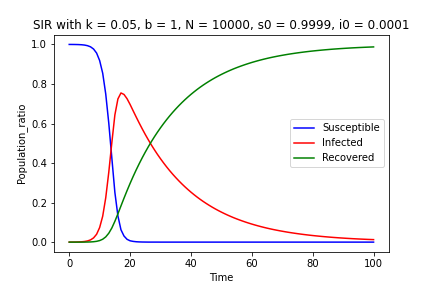
\includegraphics[scale=0.8]{sir_discrete_simulation1.png}
        \caption{A simulation of discrete SIR model in a ``socially distanced'' society.}
        \label{fig:discrete_simulation1}
    \end{figure}
    
    \newpage
    We can also use discrete model to investigate how \(b\) and \(k\) can affect the dynamics of the system. First, we look at the time for all people being infected ($s(t) = 0$). From the phase diagram in Figure \ref{fig:phase_transition_full_infection_discrete}, we can draw the similar conclusion as the ODE version that large \(b\) and small \(k\) lead to the decrease of time for full infection. For small enough \(b\) and large enough \(k\), there will always be people that are not infected. The major difference between discrete and ODE results is the phase boundary. For discrete model, the boundary is more step-like and have more sudden changes along \(b\) and \(k\) axis. This is again due to the discrete change of data in discrete model. 
    
    \begin{figure}[h!]
        \centering
        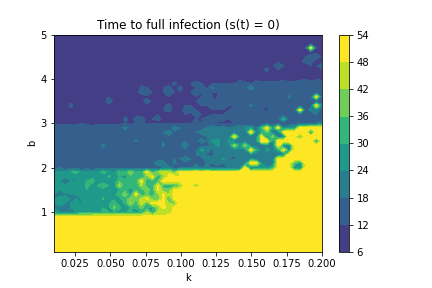
\includegraphics[scale=0.8]{phase_transition_full_infection_discrete.png}
        \caption{Phase diagram relating parameters and time to full infection for discrete model.}
        \label{fig:phase_transition_full_infection_discrete}
    \end{figure}
    
   Finally, we can take a further look at the scenario where the infected people prevail in number($i(t) > 0.5$). Similar to Figure \ref{fig:phase_transition_outnumber}, we can see that the phase boundary for discrete model, as shown in Figure \ref{fig:phase_transition_outnumber_discrete}, shifts towards smaller \(b\) and larger \(k\) values, which again indicates that there are some instances where $i(t) > 0.5$ is fulfilled while $s(t) > 0$.
    
    \begin{figure}[h!]
        \centering
        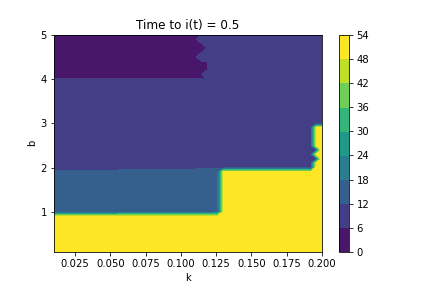
\includegraphics[scale=0.8]{phase_outnumber_discrete.png}
        \caption{Phase diagram relating parameters and time to \(i(t) > 0.5\) for discrete model.}
        \label{fig:phase_transition_outnumber_discrete}
    \end{figure}
    \newpage
    
    \section{Proposed variations}

    \subsection{Reinfection and spatial structure: a continuous SIRS model}
    Many diseases do not grant immunity to those who have recovered after being infected. In the case of viral infections, there are often different strains in the population at the same time. Those who have been infected once by one strain can be infected again with the other strain. One can then pose the interesting question: when is a disease completely eradicated from a population, and when does the disease recur? 
    
    To model reinfection, we can modify the SIR model to obtain the SIRS model in which individuals who are in the recovered group can transition to the susceptible group. We introduce a new parameter \(m\) to denote the rate at which recovered individuals become susceptible \cite{brauerCompartmentalModelsEpidemiology2008}. (Here, \(m\) stands for mutation with the interpretation being that recovered individuals become susceptible as the pathogens mutate.) Modifying the SIR model, we obtain the following system of coupled differential equations 
    \begin{align*}
        s'(t) &= -b\cdot s(t) \cdot i(t) + m\cdot r(t) \\
        i'(t) &= b \cdot s(t) \cdot i(t) - k\cdot i(t) \\
        r'(t) &= k \cdot i(t) - m \cdot r(t).
    \end{align*}
    To cast our earlier questions in the context of this model, we can ask the following question. For which configurations of the parameters \((b,k,m)\) do we get \(i(t) = 0\) at some time point \(t\) (i.e. disease is eradicated)? For which configurations do we have \(i(t) > 0\) for all time points \(t\) (i.e. disease is endemic)?

    As stated, this model posits that any individual in the infected group can interact with any individual in the susceptible group. This is not a realistic assumption as people only interact with people who are nearby. In particular, interactions are spatially structured, and this spatial structure has implications for how fast the disease can spread \cite{ducasseQualitativePropertiesSpatial2020}. This spatial structure will have real implications for simulating disease spread at large geographical scales (such as the spread within a country or a continent rather than just a city or a town). To account for this, we modify the SIRS model and define a two dimensional spatial SIRS model \cite{baileySimulationStochasticEpidemics1967}. We obtain the following system of differential equations 
    \begin{align*}
        \frac{\partial s(x,y,t)}{\partial t} &= -b \cdot s(x, y, t) \cdot \widetilde{i}(x, y, t) + m \cdot r(x, y, t) \\
        \frac{\partial i(x, y, t)}{\partial t} &= b \cdot s(x, y, t) \cdot \widetilde{i}(x, y, t) - k \cdot i(x, y, t) \\
        \frac{\partial r(x, y, t)}{\partial t} &= k \cdot i(x, y, t) - m \cdot r(x, y, t)
    \end{align*}
    where 
    \begin{equation*}
        \widetilde{i}(x, y, t) = \int_{\mathbb{R}^2} \frac{1}{\sqrt{2\pi \tau^2}} \exp\left(-\frac{(x-x')^2 + (y-y')^2}{2\tau^2} \right) \, dx' \, dy'.
    \end{equation*}
    In this model, the susceptible individuals at location \((x, y)\) at time \(t\) interact with infected people at other locations at time \(t\) with weights exponentially decaying in the distance to those other locations. The parameter \(\tau^2\) determines the ``interaction length". 

    With this model, we can then investigate how travel restrictions affect disease spread. A travel restriction corresponds to a decrease in the value of \(\tau^2\). For a choice of \((b, k, m)\) we can ask whether there are choices of \(\tau^2\) that lead to the disease being eradicated. Moreover, we can investigate the relative importance of social distancing vs travel restrictions, i.e. what is the interplay between \(b\) and \(\tau^2\)? 

\subsection{The effects of 'lock down' on disease spread: an agent-based SIRS model}
In face of the outbreak of Covid-19, social distancing interventions or more strict 'lock down' measurements are introduced to slowdown the spread of the disease. Although people in principle agree on the necessity of this measurement, in many western countries, many questions around it is still under debate even today. These questions include when to introduce 'lock down', how strict it should be, how long we should remain in 'lock down' or quarantine, and etc. To demonstrate the effects of 'lock down' on the dynamics of disease spread and shed light on the questions mentioned above, we propose to use a simple agent-based (discrete) SIR model to simulate the evolution of the disease.

To achieve this goal, there are some modifications needed to be added to the basic SIR model. In current model, each people can interact with $b$ people to potentially transmit the virus, which is not realistic since people should only interact with those who are nearby. Thus, in order to introduce the spatial structure into the model, we transfer the discrete model onto a 2 dimensional grid with length $L$. You can image it as a country with area $L \times L$. And people can now only interact with each other when they are within a distance of $D_0$. By tuning this new parameter $D_0$, we can now mimic the effects of 'lock down' measurement \cite{kaxiras2020multiple}. 

For example, we can make $D_0$ time-dependent \cite{kaxiras2020multiple}:
\begin{equation}
\label{D0}
D_{0}(t)=\left\{ \begin{array}{lcl}
D_0 & \mbox{for}
& t \leq T_0  \\
D_{0}e^{-(t - T_0)/\lambda} & \mbox{for} & t > T_0
\end{array}\right.
\end{equation}
The $T_0$ represents the timing of 'lock down' while the $\lambda$ represents how fast the 'lock down' take into effect. Assuming $\lambda > 0$, as $t \to +\infty$, $D_0 \to 0$. Thus, people are being confined into a small place and cannot affect each other. By changing $T_0$ and $\lambda$ and monitoring how the three types of population evolve with time, we can then answer the questions relate to the effects of 'lock down'.

Furthermore, we can set a time $T_1$ when we release the 'lock down' measure and $D_0(T_1) = D_0$ to see how the pandemic will evolve if we end 'lock down' too early. Along with these parameters, we can also tune $b$ to simulate the effectiveness of wearing masks or social distancing on slowing down the spread of disease. To present the results, some 2 dimensional phase diagrams can be useful. For agent-based simulation in grid, short animation illustrating how the infected population evolves (showing by color dots) can be very powerful.

\subsection{SIR model that depends on current state}
    In reality, a single system of odinary differential equation might not accurately capture the patterns in changes of \(s(t)\), \(i(t)\) and \(r(t)\) throughout the process. For example, when a significant size of the population are infected, the government intervention and media exposure to the virus may potentially alter people's behavior. Moreover, after medical supplies are allocated and feasible treatment has been found, infected people may recover quicker. In these situations, once \(i(t)\) or \(r(t)\) reaches a certain threshold, there is foundamantal changes to the systems of differential equations. In particular, the parameters \(b\) and \(k\) would change in response to the real world incident, and the system of equation now becomes
    \begin{align*}
        s'(t) &= -b'\cdot s(t) \cdot i(t) \\
        i'(t) &= b'\cdot s(t) \cdot i(t) - k'\cdot i(t) \\
        r'(t) &= k'\cdot i(t)
    \end{align*}
where
    \begin{align*}
       b' < b \\
       k' > k
    \end{align*}
in the discussion above. Using this model, we would be able to see the effects of public policies in the middle of simulation. We may want to answer, given a fixed initial condition, how does the time such alternation occur impact the peak of infection. Given the effectiveness of a policy or treatment (fix \(b'\) and \(k'\)), what would be the last day for such alternation to take place in order to cap the maximum infected population under certain threshold for various initial conditions? One way to answer these questions is to set an event such as  \(i(t) = 0.1\), which terminates the original ode simulation, and run a different simulation with the new parameters for the remaining time interval. Further analysis would be based on the concatenated solution of the two systems.

\subsection{"Light at the end of the tunnel: SIRV model"}

	With the exciting announcement from the biotech companies Pfizer and BioNTech that Covid-19 vaccines with 90 percent efficacy will soon be available to be used, one might ask how introducing 'vaccinated people' into the model will change the dynamics we saw in discrete disease spread model. Vaccines will not only slow down the spread of infectious disease in time but it will also affect how the disease will spread in space. Change in the spatial dynamics of infectious disease might have a profound impact on how quickly disease will spread in time, so one might also wonder what might be the most effective way of delivering vaccines in space.
	In this variation, we will perform a simulation where we introduce 2-dimensional grid that represents 2-dimensional space and the vaccines to the existing discrete disease spread model. The 2D grid will be populated with the three groups of people as before but they now have four possible internal states: SIRV where V stands for vaccinated. Each person will be stationary (mimicking maximum social distancing) throughout the simulation but will interact with its immediate neighbors (maximum 8 neighbors). We propose to simulate a few different scenarios in which the vaccines are delivered in slightly different ways.
	1. Targeted vaccination: In the idealized targeted vaccination scenario, vaccines will be delivered only to those who have not yet been infected (but susceptible). 
	2. Random vaccination: In this more chaotic scenario, people claim for an equal right to be vaccinated regardless of their internal states.  
	3. Does prioritizing specific locations to "drop" the vaccines in 2D grid matter for how fast the disease will spread? It is conceivable that more evenly distributed vaccination will be more effective in preventing the disease from spreading. We propose to simulate two possible scenarios where vaccines will be available either at random in space or predefined "hot spots" given the constraints defined in scenario 1 and 2. 
	A possible approach to implement this is to create a 2D grid where each cell is a class representing a person with a randomly assigned internal state. A simulation will keep track of the internal states over time, changing them by a rule that is a function of internal states, space as well as the conditions and constraints defined above. To compare and contrast the spatial and temporal dynamics of disease spread under different conditions more effectively, we will provide animated figures.	

    \bibliographystyle{unsrt}
    \bibliography{disease}

\end{document}
